\section{Experiment}
Experiment aims at using reinforcement learning algorithms for solid-state lidar with steerable rays and limited number of rays. At first it was necessary to create environment where the agent can learn and evaluate \cite{rozsypalek2018}. Lidar-gym environment is written in python 3 based on OpenAI gym interface \cite{openai2016}. It uses point clouds from Kitti dataset drives\cite{geiger2013}. One episode of learning in environment corresponds to one drive in Kitti dataset. Large point clouds from drives are processed into 3D voxel maps by C++ package \cite{petricek2017}, which also provides ray tracing engine for environment. Every voxel map is 3D array containing real numbers which corresponds to the occupancy $c$ of each voxel.
\begin{align}
\begin{split}
c &> 0 \quad \text{occupied voxel} \\
c &= 0 \quad \text{unknown occupancy} \\
c &< 0 \quad \text{empty voxel.}
\end{split}
\end{align}
Environment also offers visualisation of actions using Mayavi \cite{mayavi2011} and ASCII art. Agents use neural networks as function estimators, which are handled by Tensorflow \cite{tensorflow2015} and Keras \cite{keras2015}.

\subsection{Environments}
Lidar-gym implements several environments, which follow same template with different sizes. Observation space is local cutout of voxel map, which provides occupancies from sensor sparse measurements. Sensor is located in quarter of x axis and half of y and z axis of local cutout. Action space is divided into two parts. First part is dense voxel map reconstructed from observations (sparse measurements). Second part of action space are directions of measuring rays. Each ray has own azimuth and elevation. Environment expects directions in format of 2D array of booleans, where true means fired ray. Environments reward is negative logistic loss $-L$ \eqref{eq:loglos}. Lidar-gym defines environments with parameters described in table \ref{tab:envs}.

\renewcommand{\thefootnote}{\fnsymbol{footnote}}

\begin{table}[h]
\centering
\begin{tabular}{|c||c|c|c|} 
\hline
Name of environment     & Large                        & Small                        & Toy                       \\ \hline
Voxel map size [voxels] & 320 $\times$ 320 $\times$ 32 & 160 $\times$ 160 $\times$ 16 & 80 $\times$ 80 $\times$ 8 \\ \hline
Lidar FOV [\textdegree]           & 120 $\times$ 90              & 120 $\times$ 90              & 120 $\times$ 90           \\ \hline
Densitiy of rays        & 160 $\times$ 120             & 120 $\times$ 90              & 40 $\times$ 30            \\ \hline
Lidar range [m]         & 42                           & 42                           & 42                        \\ \hline
Number of rays          & 200                          & 50                           & 15                        \\ \hline
Voxel size [m] & 0.2 & 0.4 & 0.8 \\ \hline
Episode training time [min]\footnotemark{} & 120 & 15 & 1.5 \\ \hline
\end{tabular}
\caption{Environment description}
\label{tab:envs}
\end{table}
\footnotetext[1]{Using GPU Nvidia 1080Ti.}
\clearpage
Due to the high time complexity were all experiments conducted in toy environment. RL agents need significantly more training steps than supervised agents. In OpenAI baselines \cite{openai2017} are RL agents trained for over million timestamps. One drive in Kitti dataset has on average 200 timestamps. All agents was trained and evaluated on different  drives from city part of dataset.

\subsection{Mapping agent}
Mapping agent is based on work of Zimmermann et al \cite{zimmermann2017}. It uses convolutional neural network (CNN) for reconstructing dense map from sparse measurements. 3D convolutional layers are used to learn the features and max pooling layers to avoid overfitting. Whole CNN architecture is described in figure \ref{fig:supervised}.
\vspace{3mm}
\begin{figure}[!h]
\centering
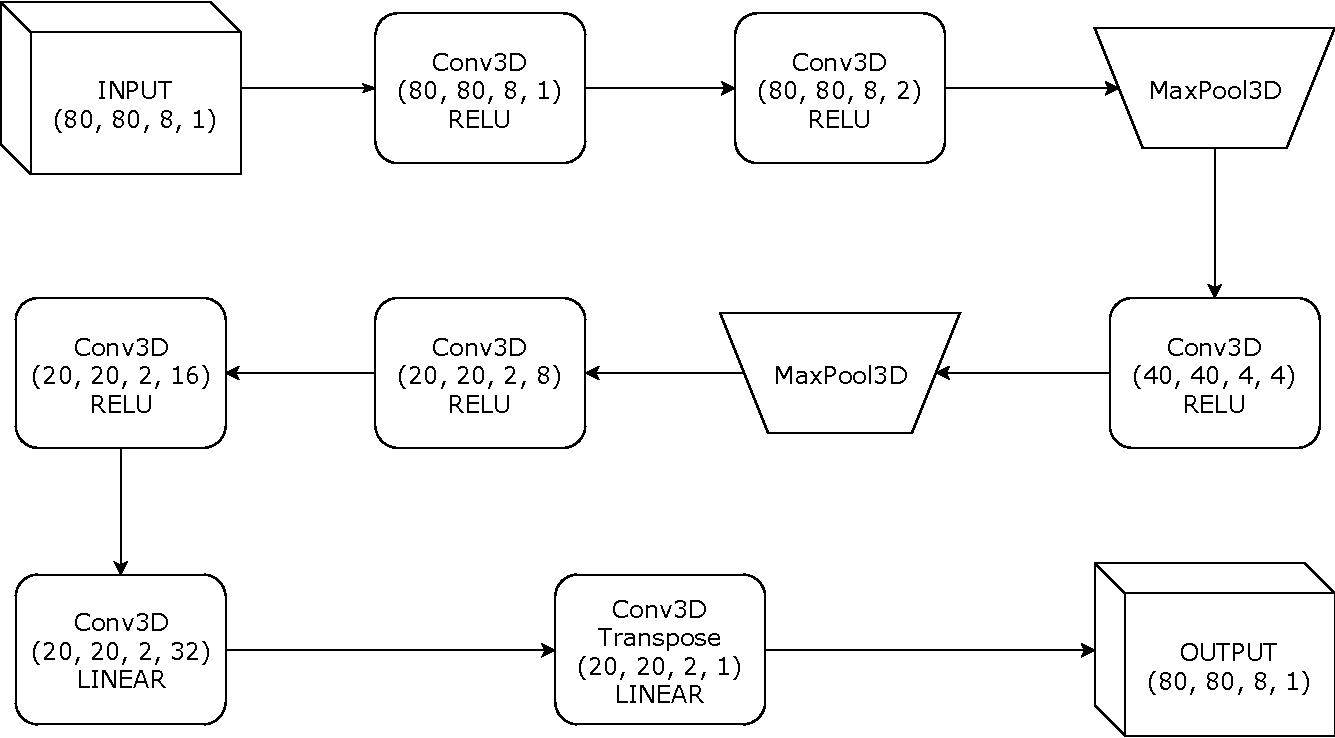
\includegraphics[scale=0.6]{fig/supervised.pdf}
\caption{Mapping network architecture}
\label{fig:supervised}
\end{figure}

For gradient descent is used logistic loss $L$ between ground truth map $Y$ and predicted dense map $\hat{Y}$.
\begin{equation} \label{eq:loglos}
L(Y, \hat{Y}) = \sum\limits_i w_i \log(1 + \exp(Y_i \hat{Y_i}))
\end{equation}
where $w$ are weights which balance importance of occupied and unoccupied voxels.
\pagebreak
Unfortunately naive implementation of this loss function is computationally inconvenient and often cause numerical issues as underflow or overflow. To stabilize training following modified loss was used \cite{matconvnet2015}.
\begin{align} 
\begin{split}
a_i &= Y_i \hat{Y_i} \\
b_i &= \max(0, a_i) \\
L &= \sum\limits_i w_i (b_i + \log(\exp(-b_i) + \exp(a_i-b_i))).
\end{split}
\end{align}
At first we train mapping agent with random ray planning. Reconstructions of supervised agent are then used for training RL planning agents and after that is mapping agent retrained with RL agent picking the rays.
\subsection{Discrete planning agent}
Insomuch as environment input for direction of the rays is 2D binary array, first try is to use discrete agent. DQN is the most used option for discrete action space but in this use case it requires some tweaks. Note that number of possible actions is extremely large. Even in toy environment it is $40\times30 \choose 15$ $\approx 10^{34}$ of actions. Thus is necessary to emphasize on action space exploration. Further arises problem with $\epsilon$-greedy policy, because we are unable to process all possible actions and pick one with the biggest Q-value. To solve this issue is considered one ray as an action and for $K$ rays is TD from \eqref{eq:qlearn} now computed as:
\begin{align}
q(S_t, A_t) &= \max\limits_{A_t}^K Q^\theta(S_t, A_t)\\
\delta_t &= R_t + \gamma \overline{q}(S_{t+1}, A_{t+1}) - \overline{q}(S_t, A_t)
\end{align}
where $\overline{q}$ is average $Q$ value over $K$ actions with maximal $Q$ values. DQN agent implements all available features described in theoretical part of this thesis as Prioritized experience replay, target network and double Q learning. Exploration is ensured by action space noise. Parameter values of agent are shown in table \ref{tab:dqlparam} and neural network architecture in figure \ref{fig:dqn}. For gradient descent is used Adam optimizer.

\begin{table}[H]
  \centering
  \begin{tabular}{*{2}{c}}
    \toprule
    Parameter & Value \\
    \midrule
    $\gamma$ & X \\
    $\alpha$ & X \\
    $\tau$ & X \\
    $\epsilon_d$ & X \\
    \bottomrule
  \end{tabular}
  \caption{Parameters of DQL agent}
  \label{tab:dqlparam}
\end{table}
\pagebreak

\vspace{3mm}
\begin{figure}[!h]
\centering
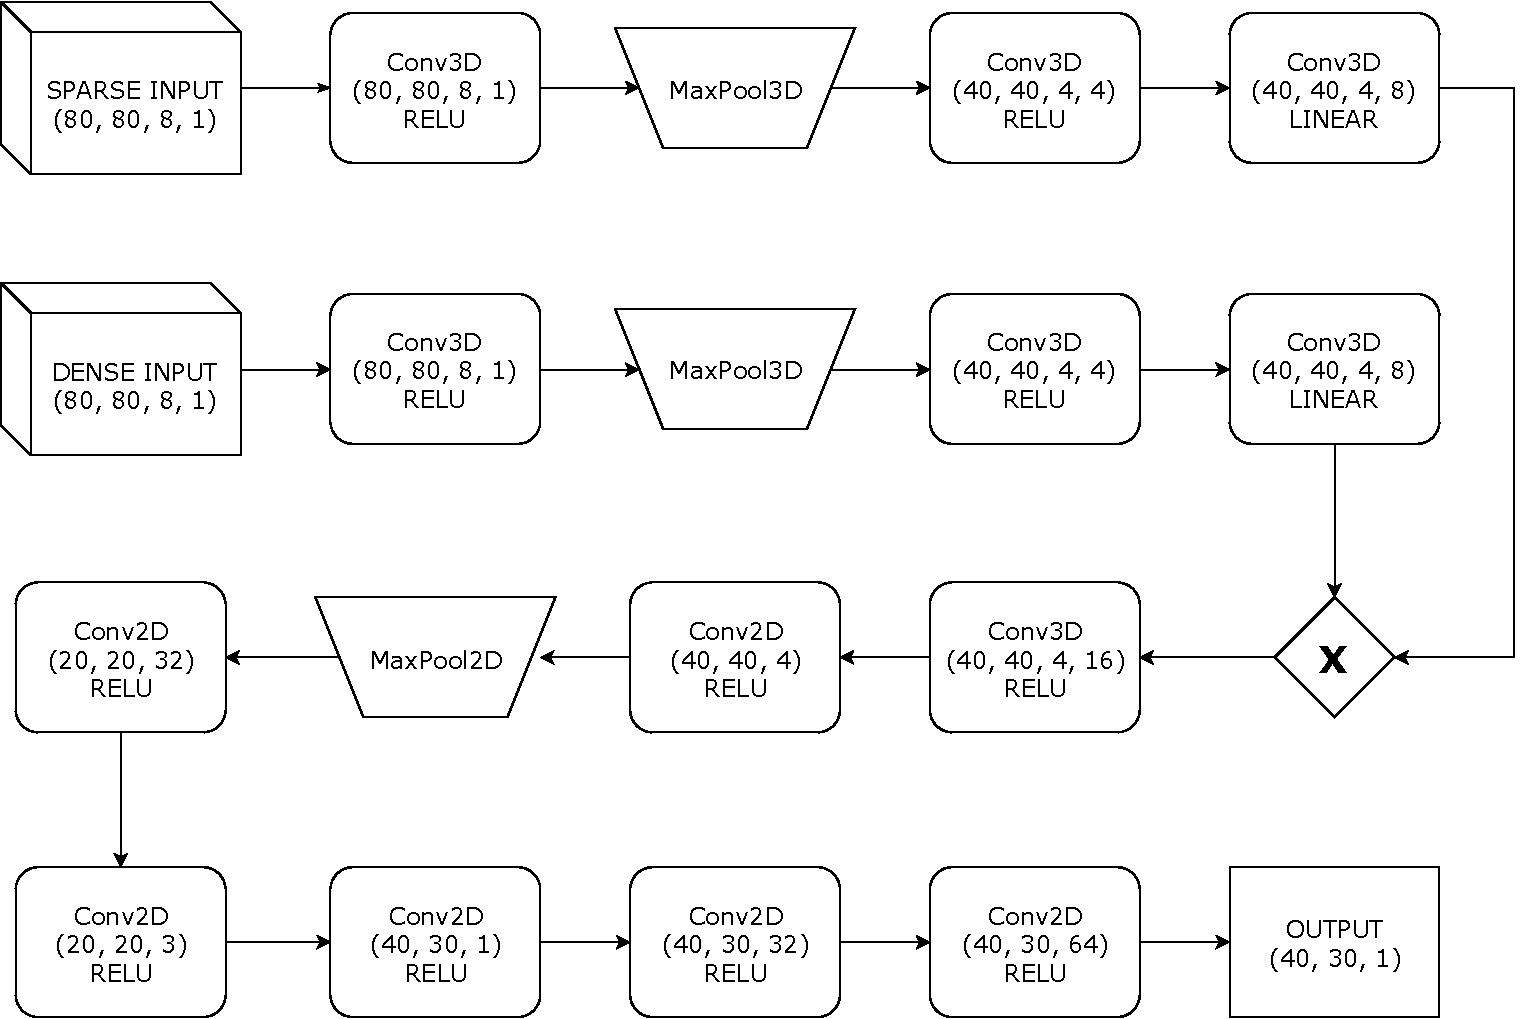
\includegraphics[scale=0.6]{fig/dql.pdf}
\caption{DQN architecture}
\label{fig:dqn}
\end{figure}

\subsubsection{Wolpetinger policy}
Wolpetinger policy is currently state-of-the-art method for discrete action spaces, because it utilize actor-critic continuous methods. It was tested on recommender systems with over a million discrete actions \cite{dulac2015}. That is large action space, but significantly smaller than action space of Lidar-gym environment. Obvious problem comes in place during action embedding in formula \eqref{eq:knn}. It is not possible to compute KNN with so many possible actions. When is KNN substituted by picking rays with highest value, agent does not converge well. It abandons some rays very soon and get stuck in local optimum.

\clearpage
\subsection{Continuous planning agent}
To avoid extremely large actions was discrete action space substituted by continuous action, which is then mapped into 2D binary array. Thank to this change it is possible to exploit actor-critic framework. Output of actor is now $2$ by $K$ array where first row is the elevation and second is the azimuth of each ray. Last layer of the actor network is tanh function, so its output is element of $[-1, 1]$. As training algorithm is used DDPG. To explore action space correctly it is necessary to apply Ornstein-Uhlenback random process. When we use only normal distribution for action space noise, actions tend to converge into the corners very fast.